% !TEX root = main.tex

\section{IO管理与磁盘调度}
控制设备和内存或CPU之间的数据传送方式:
\begin{itemize}
    \item 程序控制(programmed IO)
    \item 中断驱动方式(interrupt-driven IO)
    \item 直接内存访问(Direct Memory Access, DMA)
\end{itemize}

假脱机技术(Simultaneous Peripheral Operations On Line, SPOOL)/虚拟设备技术:
专门利用一道程序来完成对设备的IO操作,而无需使用外围IO处理机
\begin{figure}[H]
    \centering
    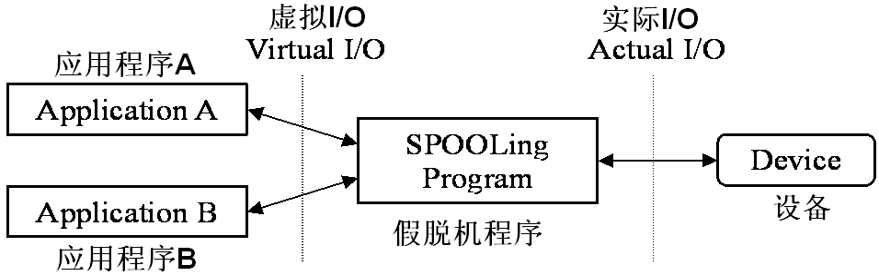
\includegraphics[width=0.7\linewidth]{fig/SPOOLing.png}
\end{figure}
优点是高速虚拟IO操作,实现对独享设备的共享

IO缓冲:
\begin{itemize}
    \item 单方向缓冲:单缓冲、双缓冲、环形缓冲
    \item 双方向缓冲:缓冲池(buffer pool)
    \item 循环缓冲
\end{itemize}

磁盘调度算法
\begin{itemize}
    \item 先进先出FIFO
    \item 优先级PRI
    \item 后进先出LIFO
    \item 最短服务时间优先(shortest-service-time-first, SSTF)
    \item 电梯算法/扫描算法SCAN
\end{itemize}